\documentclass[tikz,border=2pt]{standalone}
\usetikzlibrary{arrows.meta,positioning,calc}
\begin{document}
% Vector signal-flow diagram; the paper already loads the required TikZ libraries.
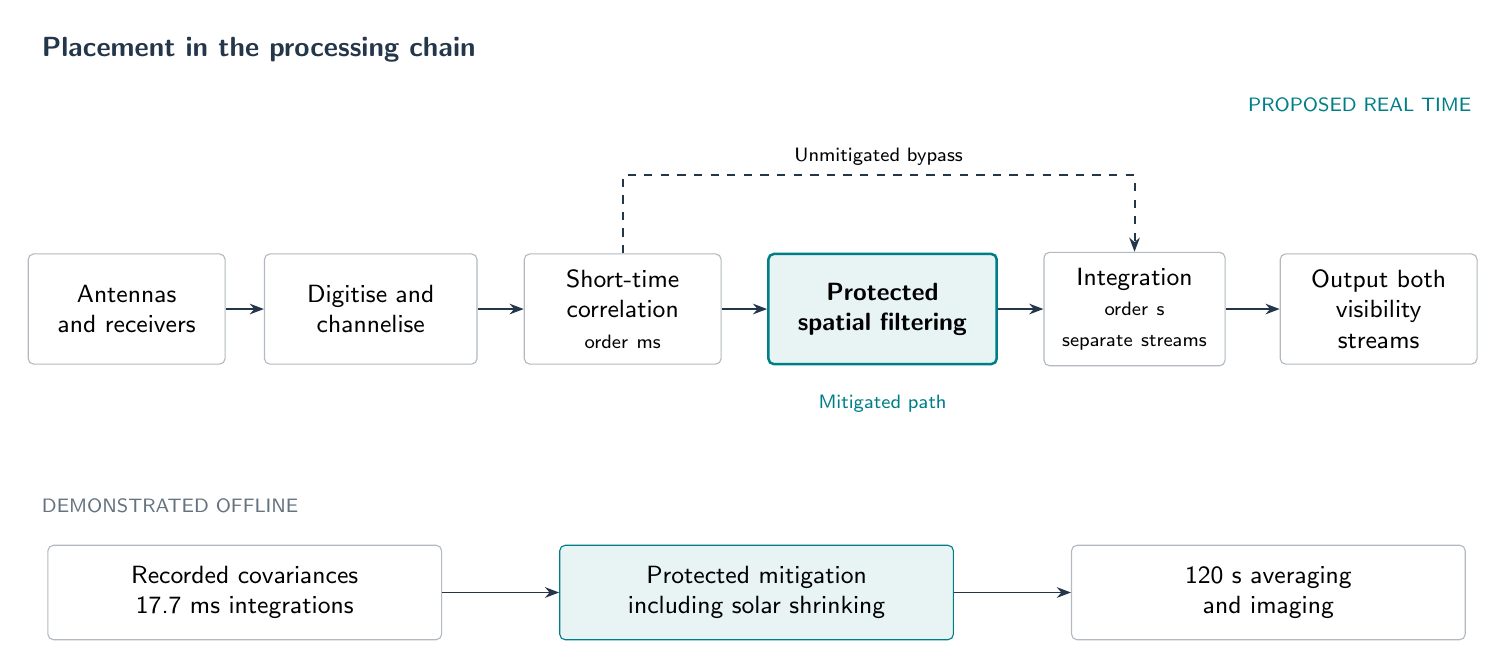
\begin{tikzpicture}[x=1mm,y=1mm,font=\sffamily\fontsize{9}{11}\selectfont,
  flow/.style={-{Stealth[length=1.8mm]},line width=.7pt,draw=ink},
  box/.style={draw=ink!35,fill=white,rounded corners=2pt,align=center,inner sep=2mm},
  small/.style={font=\sffamily\fontsize{7.5}{9}\selectfont},
  heading/.style={anchor=west,font=\sffamily\bfseries\fontsize{10}{12}\selectfont,text=ink}]
\definecolor{ink}{HTML}{23364A}
\definecolor{teal}{HTML}{007E87}
\node[heading] at (0,33) {Placement in the processing chain};
\node[small,text=teal,anchor=east] at (184,26) {PROPOSED REAL TIME};
\node[box,text width=21mm,minimum height=14mm] (front) at (12,0) {Antennas\\and receivers};
\node[box,text width=23mm,minimum height=14mm] (dig) at (43,0) {Digitise and\\channelise};
\node[box,text width=21mm,minimum height=14mm] (cov) at (75,0) {Short-time\\correlation\\{\scriptsize order ms}};
\node[box,draw=teal,fill=teal!9,line width=.9pt,text width=25mm,minimum height=14mm] (mit) at (108,0) {\textbf{Protected}\\\textbf{spatial filtering}};
\node[box,text width=19mm,minimum height=14mm] (integ) at (140,0) {Integration\\{\scriptsize order s}\\{\scriptsize separate streams}};
\node[box,text width=21mm,minimum height=14mm] (outlive) at (171,0) {Output both\\visibility streams};
\foreach \a/\b in {front/dig,dig/cov,cov/mit,mit/integ,integ/outlive} \draw[flow] (\a) -- (\b);
\draw[flow,dashed] (cov.north) -- (75,17) -- node[above,small] {Unmitigated bypass} (140,17) -- (integ.north);
\node[small,text=teal] at (108,-12) {Mitigated path};
\node[small,text=ink!70,anchor=west] at (0,-25) {DEMONSTRATED OFFLINE};
\node[box,text width=46mm,minimum height=12mm] (disk) at (27,-36) {Recorded covariances\\17.7 ms integrations};
\node[box,draw=teal,fill=teal!9,text width=46mm,minimum height=12mm] (off) at (92,-36) {Protected mitigation\\including solar shrinking};
\node[box,text width=46mm,minimum height=12mm] (image) at (157,-36) {120 s averaging\\and imaging};
\draw[flow] (disk) -- (off);
\draw[flow] (off) -- (image);

\end{tikzpicture}

\end{document}
